\documentclass[]{article}
\usepackage[margin=1in]{geometry}
\usepackage{graphicx}
\usepackage{lscape}

\begin{document}

\title{SmokeSNET Model}
\author{Matt Smith}
\date{\today}
\maketitle

\section{Current Attributes}
As it stands, nodes have the following attributes:
\begin{table}[h]
    \begin{tabular}{|l|l|l|}
        \hline
        Name & Type & Represents \\ \hline
        	isSmoker &  Boolean & True if they're a smoker, false otherwise \\ 
 	willpower &  Double & A probability representing willpower, 0 being of strong willpower \\ 
	health &  Double & A value between 0 and 1 for health, where 1 is perfect health \\ 
	smokedPerDay &  Integer & The number of cigarettes smoked per day\\ 
 	givingUp &  Boolean & True if they're giving up, false otherwise \\ 
 	stepsSinceGiveUp &  Integer & The number of simulation steps since giving up \\ 
	sociable &  Double & A probability representing how sociable someone is, with 1 being very sociable \\ 
        \hline
    \end{tabular}
\end{table}
Edges are directed and their weight is a probability, representing their influence.
Nodes can also be constrained to a maximum number of in-edges, i.e. nodes which influence them. Within each simulation step, the following happens:
\begin{enumerate}
\item The local neighbourhood within three incoming hops is acquired for the given node. Influence between the nodes is calculated as the maximum influence across all possible connections of the two nodes, where influence over multiple hops is the product of the influence of each hop. For example, in Fig. \ref{networkdiag}, the influence of \emph{Node C} on the \emph{Current Node} is the maxiumum of $0.8 * 0.8$ and $0.1$, the maxiumum value here is $0.64$ for \emph{Node C} to \emph{D} to \emph{Current}. All nodes within the neighbourhood set are unique.
\item Metrics for this set are calculated for the current node relative to the neighborhood. 
\begin{figure}[h]
\begin{center}
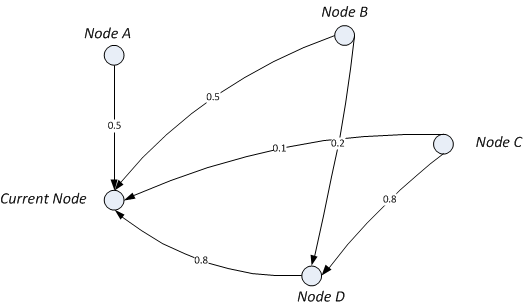
\includegraphics{networkdiag.png}
\label{networkdiag}
\caption{Network Diagram}
\end{center}
\end{figure}
\end{enumerate}
This is a work in progress - I'm planning to add the following attributes over the next few days:
\begin{itemize}
\item A representation of addiction - probably a value between 0 and 1, that can be decremented as 
\item
\end{itemize}

\end{document}